% $Id: latexforreportwriting.tex 460 2010-01-29 10:36:37Z fangohr $ 

\documentclass[12pt,a4paper]{article}

\setlength{\topmargin}{-2cm}
\setlength{\oddsidemargin}{0cm}
\setlength{\textheight}{24cm}
\setlength{\textwidth}{16cm}

\usepackage{graphicx}

\usepackage{listings}

\usepackage{sectsty}

%Use Helvetica as the sans serif font
\usepackage{helvet}                         
 
%Use sffamily for all titles
\allsectionsfont{\sffamily}

\begin{document}

\title{\sffamily \huge \textbf{ Using  \LaTeX\ for report writing}}

\date{Hans Fangohr}

\author{University of Southampton, United Kingdom}

\maketitle



\tableofcontents

\newpage

\section{Introduction}

This document provides a couple of hints that may be useful if you use
\LaTeX{} for the first time for writing a report. 

We append the source of this file should you want to study it.

The main purpose of this document is to make you aware of \LaTeX{}
commands that may be useful. It is not possible to explain all of
these on a few pages. Instead, you should understand this document as
a help providing pointers to ``interesting'' commands which you can
then look up in other documentation.

We also assume that you have a basic understanding of latex (and have
worked through the latex exercises in your computing module).

\section{Including figures}

The exercises in laboratory session 4 provide an example of how to
create an eps file, and how to include this file into a \LaTeX{}
document. Take this as a starting point.

\subsection{How do I include Matlab graphs into my LaTeX document?}

When you have created the figure, use the \texttt{print -depsc2
  filename.eps} command to create an eps file with name
\texttt{filename.eps} to contain that figure.

\subsection{How do I include Pylab graphs into my LaTeX document?}

Either use \texttt{pylab.savefig('myfilename.eps')} to save the file,
or click on the disk icon on the figure window, and chose ``eps'' as
the filename extension. Then proceed as usual.

If you like to save the picture as a ``png'' or ``pdf'' file, just use
``png'' or ``pdf'' as the file name extension (for pdflatex).


\subsection{How do I include Visual Python Snap shots into my LaTeX
  document?}
\label{sec:vpythontoeps}

Visual Python is meant to be a real-time 3d visualisation system and
is not designed to save high-quality graphs. We can still create
visual python eps files but it takes several steps.

With the software tools we have available at the university, this
seems the easiest approach to create eps files from Visual Python
windows:
\begin{enumerate}
\item Bring the Visual Python Window you want to save to a file on the
  screen. Make the figure window as large as possible (this will
  increase the resolution of your figure).

\item Capture the figure by
  \begin{itemize}
  \item clicking on the figure window with the mouse and

  \item pressing Alt+"Print Screen" (this copies the figure into the
    clip board)
  \end{itemize}

\item  Now we need to convert the captured bitmap into an eps file
  \begin{enumerate}
  \item Start Corel Draw (Start $\rightarrow$ All Programs
    $\rightarrow$ Graphical $\rightarrow$ Corel Graphics $\rightarrow$
    Corel DRAW)

  \item  click on "New"

  \item  Edit$\rightarrow$Paste
  \item  File$\rightarrow$Export
  \item  select desired directory for saving the file

  \item select "Save as type" to be "EPS"

  \item click "Export"
  \end{enumerate}
\end{enumerate}
You should now find an eps file with the name of your choice on
disk. Make sure you copy this file to the directory with your LaTeX
file so that LaTeX can find the figure file when it compiles your
document.

(Coreldraw can also export PNG files if you want to convert your
Visual Python figures to this format [for example to place the figures
into MicroSoft Word, or for use with pdflatex]. However, if you don't
need eps files, then the [simpler] MS Paint programm is sufficient for
step 3.)


\subsection{How to convert other graphic file formats to eps files}
\label{sec:conversiontoeps}

Open the file in Corel draw and export to EPS. See \ref{sec:vpythontoeps}


\section{Including listings (source code)}

If you want to include source code, you should use the Type-wriTer
(TT) font. (In MS Word, this font is called Courier.) The advantage of
the TT-font (over the standard font we use to write the main text) is
that every character has the same width, including dots and spaces.

Generally, it looks better if the (horizontal) space a letter or
symbol occupies varies with its width. For example, 20 \emph{i}
letters (iiiiiiiiiiiiiiiiiiii) will need less horizontal space than 20
\emph{m} letters (mmmmmmmmmmmmmmmmmmmm). However, for printing source
code we want to align rows (independent of what letters are being
used) to adequately represent indentation. We also do not want to
\LaTeX{} to typeset the source! Therefore, \LaTeX{} provides a special
environment for this. It is called ``verbatim''.


\subsection{The verbatim environment}

\subsubsection{Standard use}

In the verbatim environment, \LaTeX{} will typeset everything exactly
as being written in the \LaTeX{} source file, including spaces and
linebreaks. It uses a fixed-width font for this. Suppose we want to 
include this listing of a function that (recursively) computes n
factorial:
\begin{verbatim}
function answer = fac(n)

if n == 1
    answer = 1
else
    answer = n*fac(n - 1)
end
\end{verbatim}

To achieve this, you have to include the following in the \LaTeX{}
source file
\begin{verbatim}
\begin{verbatim}
function answer = fac(n)

if n == 1
    answer = 1
else
    answer = n*fac(n - 1)
end\end{verbatim}\verb:\end{verbatim}:\\ 
%have to cheat here to get \end{verbatim} printed
                                         

In other words, the sourcecode has to be enclosed by
\verb:\begin{verbatim}: in the beginning and \verb:\end{verbatim}: in
the end.

\subsubsection{Using other font sizes in verbatim environment ---
  option 1}


If you want to include a long listing, you may wish to slightly reduce
the size of the font. You can do this by switching to a smaller font
before the verbatim environment (for example using \verb:\small: or
\verb:\footnotesize:) and switching back to the normal font size after
the environment (using \verb:\normalsize:). You have to change the
font size \emph{outside} the verbatim environment, otherwise the
command will simply be printed (but not executed).

Here is an example using the \verb:\footnotesize: command:
\footnotesize
\begin{verbatim}
function answer = fac(n)

if n == 1
    answer = 1
else
    answer = n*fac(n - 1)
end
\end{verbatim}
\normalsize

which was created using the following commands in the \LaTeX{} file

\begin{verbatim}
\footnotesize
\begin{verbatim}
function answer = fac(n)

if n == 1
    answer = 1
else
    answer = n*fac(n - 1)
end\end{verbatim}\verb:\end{verbatim}:\\ 
%have to cheat here to get \end{verbatim} printed
\verb:\normalsize:

\subsubsection{Using other font sizes in verbatim environment ---
  option 2}

There is a danger to forget to switch back to the normal size font
(and then all subsequent text will be printed in footnote size until
the next font size changing command is encountered). This can be
avoided by including the \verb:\footnotesize: command and the verbatim
environment in curly braces as shown here:

\begin{verbatim}
{ \footnotesize
\begin{verbatim}
function answer = fac(n)

if n == 1
    answer = 1
else
    answer = n*fac(n - 1)
end\end{verbatim}\verb:\end{verbatim}:\\ 
%have to cheat here to get \end{verbatim} printed
\verb:}:

Here it is important not to forget the closing curly brace after the
\verb:\end{verbatim}: command.


\subsection{The verb command}

If you want to print a single word or character in the same font as
the verbatim environment, or if you want to print a \LaTeX{} command,
then you can use the ``verb'' command. The syntax is as follows:

\verb:\verb X TEXTTOBEPRINTED X:

The letter \verb%X% can be substituted by any symbol such as :,
\verb:!:, \verb:|:, \verb:#: as long as this symbol is not used 
within the command to be printed. The symbol is used to indicate 
the beginning and the end of the string. Here are some examples:

\noindent The command\\ \verb:  \verb!\large!:\\ will print 
\\\verb!  \large!,\\ the command\\ \verb|  \verb:rhsho.m:|\\ 
will print\\\verb:  rhsho.m: 




\subsection{The listing environment}
\label{sec:listing}

There is an extension package to LaTeX (which is available on the
machines of the university) which is written especially to type set
source code nicely. It comes with a number of features including
keyword highlighting and framing source code. The full documentation
is coming with the software (homepage:
\texttt{www.atscire.de/products/listings}).

In the preamble of your document (i.e. before
\verb:\begin{document}:), you need to include the package:

\begin{verbatim}
\usepackage{listings}
\end{verbatim}

\lstset{frame=tlrb}
\lstset{basicstyle=\ttfamily\footnotesize}

You can then set some default options for the layout of the source
code (this can be in the preamble or in the main text). For example
\begin{itemize}
\item choose the default layout to use tt-family font (this is type
  writer style) and to make it printed the same size as footnotes
  (slightly smaller than normal):
\begin{verbatim}
\lstset{basicstyle=\ttfamily\footnotesize}
\end{verbatim}

\item draw a frame around the source. 
\begin{verbatim}
\lstset{frame=tlrb}
\end{verbatim}
The letters
stand for Top, Left, Right and Bottom. Just using \texttt{tb} will
give you lines on top and bottom.
\end{itemize}

We can now format some code with these settings. For example, these
lines:
\begin{verbatim}
\begin{lstlisting}
.... insert source code to be formatted here ...
\end{lstlisting}
\end{verbatim}
generate this output:
\begin{lstlisting}
.... insert source code to be formatted here ...
\end{lstlisting}

We can also include a listing from a source file. This is particularly
useful because the listing will changed (when you run LaTeX again)
after the source code has changed.

As an example, we include a part of this file into itself. This latex
command
\begin{verbatim}
\lstinputlisting[firstline=6,lastline=15]{reportwriting.tex}
\end{verbatim}
results in this output:
\lstinputlisting[firstline=6,lastline=15]{reportwriting.tex}

The \texttt{firstline} and \texttt{lastline} commands are optional.
Other useful options are \texttt{numbers=left} which will print
numbers on the left-hand side of the source:

\begin{verbatim}
\lstinputlisting[numbers=left,firstline=6,lastline=15]{reportwriting.tex}
\end{verbatim}
results in this output:
\lstinputlisting[numbers=left,firstline=6,lastline=15]{reportwriting.tex}


\section{Some equations}

\subsection{Vectors}

To typeset vectors, you can use an arrow above the variable, for
example $\vec{x}$ (\verb:\vec{x}:). We recommend to follow the
convention to use boldface letters in printed materials for vectors:
$\mathbf{x}$ (\verb:\mathbf{x}:). We have provided the corresponding
\LaTeX{} command in parentheses. Remember (lab session 4 and lecture
on \LaTeX) that you need to switch to math mode first before you can
use these commands. For in-line equations, use \verb:$: %$
to switch the math mode on and off. For displayed equations (see
below), use \verb:$$:. If you want your equations to be numbered, then
you have to use the equation environment and begin the equation with
\verb:\begin{equation}: and end it with \verb:\end{equation}:.
        
Should you want to write something like 
$$ \mathbf{x} = \left( \begin{array}{c} x_1 \\ x_2 \end{array} \right) $$
then you can use the following command:

{\small
\begin{verbatim}
$$\mathbf{x} = \left( \begin{array}{c} x_1 w\\ x_2 \end{array} \right)$$
\end{verbatim}
}\bigskip

Although you can use this line (and simply substitute
\verb:\mathbf{x}:, \verb:x_1: and \verb:x_2:) without understanding
it, we explain the different components briefly:

\begin{tabular}{l|p{10cm}}\hline
  \verb:$$: & begin displayed equation environment\\
  \verb:\mathbf{x} =: & prints $\mathbf{x} =$\\
  \verb:\left (: & prints the left (=opening) parenthesis in the 
    right size for whatever comes next\\ 
    \verb:\begin{array}{c}: & begins a vector (and components are 
      horizontally centred)\\ 
      \verb:x_1: & first component of vector\\
      \verb:\\: & signal to finish first component of vector\\
      \verb:x_2: & second component of vector\\
      \verb:\end{array}: & ends vector\\
    \verb:\right ): & prints the right (=closing) parenthesis in 
  the right size for whatever is finished (here: the vector)\\
  \verb:$$: & end displayed equation environment\\\hline
\end{tabular}\bigskip

If you want to use less space, then it is easier to write $\mathrm{x}$
like this $$\mathrm{x} = (x_1,x_2)$$ using this command
\verb: $$\mathrm{x} = (x_1,x_2)$$:

{\footnotesize( Note that strictly speaking $\mathrm{x} = (x_1,x_2)$
  is not the same as $ \mathbf{x} = \left( \begin{array}{c} x_1 \\
      x_2 \end{array} \right) $ --- because the first is a row vector
  and the other a column vector. However, as long as we don't deal
  with matrices, this differences is not important and it is quite
  common to use both notations to refer to the same vector. )}


\subsection{Aligning several equations}

Should you wish to align several equations (suppose you want to
typeset a system of differential equations), the you can use the
\verb:eqnarray: enviroment for this. For example, to use the following
equations
\begin{eqnarray}
  \dot{x} &=& v\\
  \dot{v} &=& -\omega^2 x
\end{eqnarray}
you can use the following \LaTeX{} source:
\begin{verbatim}
\begin{eqnarray}
  \dot{x} &=& v\\
  \dot{v} &=& -\omega^2 x
\end{eqnarray}
\end{verbatim}

Each line is terminated by \verb:\\:. The horizontal alignment of the
different lines is chosen such that whatever is enclosed in the
\verb:&:-symbols is aligned underneath each other (here the \verb:=:
sign).


\subsection{Including text and spaces in equations}

To include (normal) text in equations, use the \verb:\mathrm{}:
command. For example, to print
$$ x^2 > x\quad \mathrm{for\:all}\quad x > 1$$
you can use \verb!$$ x^2 > x\quad \mathrm{for\:all}\quad x > 1$$!

The command \verb!\:! inserts a small space (necessary between ``for''
and ``all'' because in math mode there is no space between variables)
and \verb:\quad: inserts a big space. {\footnotesize (In fact, there
  is a symbol $\forall$ which has the meaning of ``for all'', so that
  the equation can be written as $ x^2 > x \:\forall\: x > 1$ using
  \verb!x^2 > x \:\forall\: x > 1!)}

\section{Changing margins}


\subsection{Left margin}


The default margin of \LaTeX{} for the left margin is one inch. On top
of this, an extra margin can be set, using the command
\begin{verbatim}
\setlength{\oddsidemargin}{1cm}
\end{verbatim} 
in the preamble of the document. This results in a margin of 2.54cm
(the default) plus 1cm.

\subsection{Top margin}
Similarly, the top-margin can be modified 
\begin{verbatim}
\setlength{\topmargin}{0cm}
\end{verbatim}

Note, that it is possible to use negative distances to achieve smaller
margins, for example:
\begin{verbatim}
\setlength{\oddsidemargin}{-1.54cm}
\end{verbatim} to create a 1cm margin on the left side.


\subsection{Text height and width}

Similarly, the width and height of the text can be modified using
\begin{verbatim}
\setlength{\textheight}{24cm}
\setlength{\textwidth}{16cm}
\end{verbatim}

\subsection{Line spacing}
You can also increase the line spacing by using a value greater than 1
in this command:
\begin{verbatim}
\renewcommand{\baselinestretch}{1.1}
\end{verbatim}

Remember that all the commands in this section have to be used in the
preamble of the document, \emph{i.e.} before the
\verb:\begin{document}: command.


\section{Spaces, paragraphs, pages}
Generally, you should try not to format the document yourself but to
leave it to \LaTeX{} to do this. However, there are situations where
you may wish to take explicit control and overide \LaTeX s attempts to
provide the best possible layout. The following points may be helpful
in such situations. 

\subsection{Inserting arbitrary space}

You can insert horizontal space using the \verb:\hspace: command. To
insert 1cm of horizontal space, use \verb:\hspace{1cm}:. Similarly,
\verb:\vspace{1cm}: can be used to insert vertical space.

If you want to increase the vertical spacing between two paragraphs
for some reason, you can insert ``some'' extra space (which grows and
shrinks automatically depending on the font size) using
\verb:\smallskip:, \verb:\medskip: and \verb:\bigskip:.


\subsection{Line breaking}
Should you wish to force \LaTeX{} to start a new line, you can use the
\verb:\\: command to achieve this.


\subsection{Inserting some vertical space}

You will notice that paragraphs usually start with indentation (that
is, the first line is indented). This looks good if the paragraph has 
more than 2 lines. Should you wish not to indent the first line of a
paragraph, then you can suppress this using the \verb:\noindent:
command just before the paragraph starts.

\subsection{Page breaking}

You can suggest to \LaTeX{} to start a new page at a particular point
using the \verb:\newpage: command. This is usually not necessary but
you may wish to use it when you have reached the final version of your
document and you are unhappy with the page-breaking chosen by LaTeX{}.
We do recommend not to use this command before you have finalised your
document.



\section{Special characters}
\label{sec:special}

\subsection{Control characters}

\LaTeX{} understands some characters as control characters and we have
to tell it if we want them to be 'just' printed. Two examples are
\begin{itemize}
\item the percentage sign ``\%''. To print this we have to type
  ``\verb:\%:''. The backslash is necessary to tell \LaTeX{} that it
  should print the percentage sign rather than it indicating the
  beginning of a comment in the \LaTeX{} source code.
\item the underscore ``\_''. This is used in \LaTeX{} math mode for
  subscripts. if you use it outside the math mode, then \LaTeX{} will
  complain (it seems to assume that you forgot to switch on math
  mode). To get around this, we preceed it by a backslash:
  ``\verb:\_:''.
\end{itemize}


\subsection{Other symbols}

\begin{itemize}

\item The symbol for "degree": You get a circle using
  \verb:$\circ$:. Now we need to make this a superscript using
  \verb:^:. Here is a complete example to express that the temperature
  is 3 degree Celsius:
\begin{verbatim}
The temperature is $3^\circ$C.
\end{verbatim}
which produces ``The temperature is $3^\circ$C.''.
\end{itemize}


\section{Using other fonts}\label{sec:useotherfonts}
\label{sec:using-other-fonts}

LateX has three different font types: these are the 'normal' (serif)
\textrm{roman} font (as you can enforce with \verb:\textrm{test}:),
the \textsf{sans serif} font (to which you can switch with
\verb:\textsf{test}:) and the fixed width \texttt{typewriter} font
(which can be used with \verb:\texttt{test}:).

Each of these fonts can be replaced by one other font. For example, to
replace the default roman font with the ``times'' font, you would use
\begin{verbatim}
\usepackage{times}
\end{verbatim}
in the document preamble (\emph{i.e.} before the
\verb:\begin{document}: line).  The times font will automatically
  replace the roman default font (because it is a serif-font).

If you like to replace the sans serif font with, say, Helvetica, you
can use this line in the preamble:
\begin{verbatim}
\usepackage{helvet}
\end{verbatim}

\subsection{Changing the font of all section headings}
\label{sec:changing-font-all}

Often, one would like to use the helvetica font for the section
headings, and not change the normal roman font. This can be done with
the help of the SECTion STYle package:
\begin{verbatim}
\usepackage{helvet}            %load helvetica font (replaces sf font)
\usepackage{sectsty}           %load section style package
\allsectionsfont{\sffamily}    %use sf font for headings
\end{verbatim}

For this document, we have used the commands above in the preamble.

\subsection{Changing the 'normal' font}
\label{sec:changing-normal-font}

You can change the normal font to ``times'' just by loading the
package as explained in \ref{sec:useotherfonts}.

If you would like to change the normal font to sans serif font, you
have to work a bit harder (as this is unusual):

\begin{verbatim}
\usepackage{helvet}            %load helvetica font (replaces sf font)
\renewcommand{\familydefault}{\sfdefault}                         
                               %make the sf font the default font
\end{verbatim}

LaTeX does not allow you to have more than the sans serif, the serif
and the typewriter font in the same document (at least not
easily). The reason for this is that usually having too many fonts
looks messy.




\section{How to create a pdf file from latex}
\label{sec:how-create-pdf}
\label{pdffromlatex}

This section contains information on generation of \texttt{pdf} files
from LaTeX. You have two options of creating pdf files from latex. 
If your document includes no figures, then this is straight forward
and you can skip the steps described below which relate to figures.

If you have figures in your document, you need to add
\verb|\usepackage{graphicx}| to the preamble of your document to be able
to use the \verb|\includegraphics| command.

\subsection{The standard way (using \texttt{latex})} 

The ``standard'' way of including graphics into LaTeX documents is
exactly what you have learned up to now (i.e. translate tex into dvi
and convert this into ps) but can be extended to create a \texttt{pdf}
file (Figure \ref{workflow} on page \pageref{workflow} summarises this
workflow (top)):
\begin{enumerate}
\item Create \texttt{eps} files for all pictures and diagrams, for
  example \texttt{graph.eps}
\item Include these into the latex document using
  \verb|\includegraphics{graph}|. Note that you do not have to specify
  the file name extension ``\texttt{.eps}'': LaTeX will append this
  automatically.
\item Create a DVI file (and print)
\item Convert the DVI file to PostScript (and print)
\item Convert the PostScript file into a \texttt{pdf} file:
  \begin{itemize}
  \item You can use GSView to create a \texttt{pdf}-file from your
    postscript file: Open the postscript file in GSView then
  \item click on ``File$\rightarrow$Convert...'' and
  \item choose ``pdfwrite'' as the ``Device''. A resolution of 300 or
    600 dpi is reasonable, then
  \item click ``OK'' and decide where to save the \texttt{pdf} file.
  \end{itemize}
  {\footnotesize Adobe's commercial(!) ``Distiller'' software will
    also convert PostScript files to \texttt{pdf} files (and may
    achieve better compression than GSView, i.e. will create smaller
    \texttt{pdf} files). There are many other tools (in particular on
    Mac OS X and Linux to convert postscript to pdf files; most of
    which are free to use).}
\end{enumerate}

\begin{figure}[t]
  \centering
  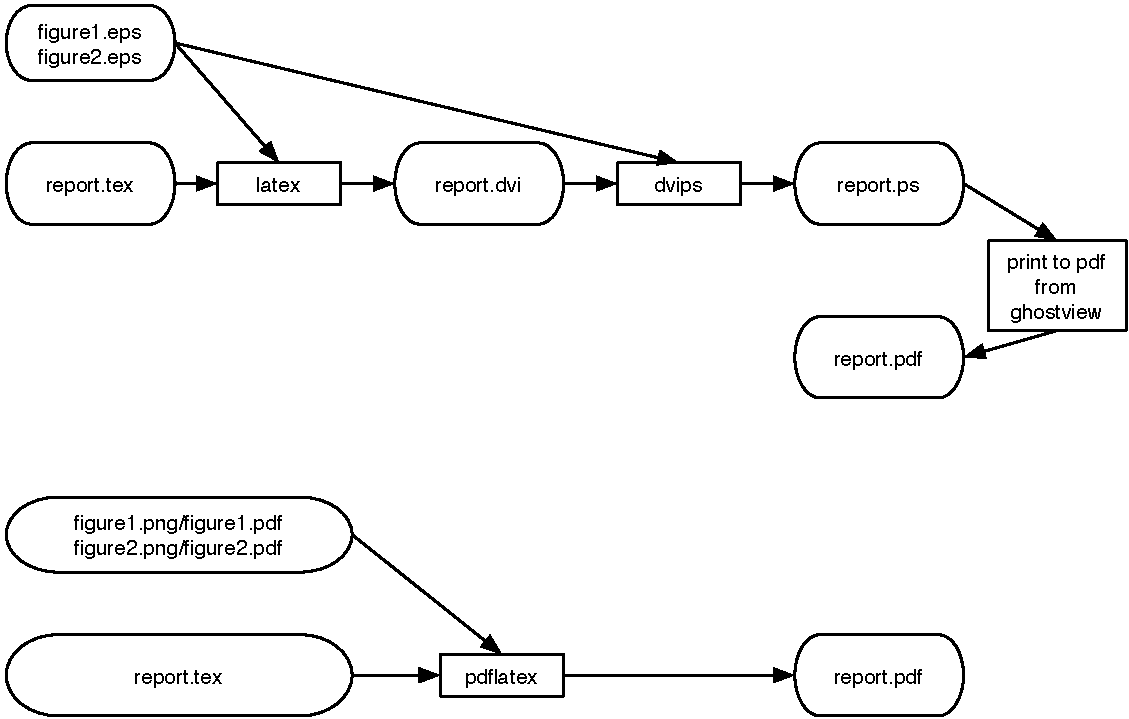
\includegraphics[width=1\textwidth]{flowdiagram}
  \caption{\emph{Top}: The standard way --- Work flow using
    \texttt{latex}, dvips and ghostview (graphics files must be in eps
    format). \emph{Bottom}: The modern way --- work flow using
    \texttt{pdflatex} (graphics files must be in pdf or png format).}
  \label{workflow}
\end{figure}


\subsection{The modern way  (using \texttt{pdflatex})}

The ``modern'' way allows to create a \texttt{pdf} file directly from
a LaTeX document (using ``PDFLaTeX''). However, if you want to do
this, then you must provide \texttt{pdf} files or \texttt{png} files
for your pictures (because \texttt{eps} files cannot be read by
PDFLaTeX). We provide the same list of instructions as above (Figure
\ref{workflow} summarises this workflow (bottom)):

\begin{enumerate}
\item Create \texttt{pdf} or \texttt{png} files for all pictures and
  diagrams, for example \texttt{graph.pdf} or \texttt{graph.png}
\item include these into the latex document using\footnote{Note that
    we have \emph{not} written \texttt{graph.pdf} or
    \texttt{graph.png}. By \emph{not} specifying the extension, we
    allow LaTeX to choose either \texttt{png}, or \texttt{pdf}
    depending on what file type is provided in the directory.}
  \verb|\includegraphics{graph}|
\item Create a \texttt{pdf} file by clicking on
  ``Execute$\rightarrow$PDFLaTeX''.
\end{enumerate}
\bigskip

\subsubsection*{Warning} 

Sometimes \texttt{pdf} viewers (such as Adobe's Acrobat) do not update
the displayed file automatically when the file changes, or (on
windows) they may block the file. This is tedious when you are still
working on the document as you will have to run PDFLaTeX again and
again to see whether you have achieved what you want to achieve.
\bigskip

\subsubsection*{Suggestion: Combining the ``standard'' and the
  ``modern'' way}

If you provide \texttt{eps} \emph{and} \texttt{png} (or \texttt{eps}
\emph{and} \texttt{pdf}) versions of all your graphic files, then you
can run the ``standard'' LaTeX and use the WinDVI viewer to design
your document. (WinDVI will automatically update the display when the
file on disk changes.) Once you are happy with the document, you can
run PDFLaTeX to generate the final \texttt{pdf} file.


\section{Summary}

This document provides links to some commands that can prove useful in
writing documents using \LaTeX. It is unrealistic to attempt to
explain them in detail on a few pages; instead we'd like to make you
aware of the existence of these commands and encourage you to look
them up in the literature.

You are welcome to ask \LaTeX{} related questions in the labs, and to
consult members of staff should you have difficulties or further
questions.



\appendix

\section{The latex source code of this document}

\lstinputlisting{reportwriting.tex}

\vfill\hrule \tiny 
$ $Id: latexforreportwriting.tex 460 2010-01-29 10:36:37Z fangohr $ $

\end{document}
